\documentclass[11pt,a4paper]{article}
\usepackage[T1]{fontenc}
\usepackage[utf8]{inputenc}
\usepackage{lmodern,amsmath,amssymb,booktabs,array,tikz}
\usepackage[margin=25mm]{geometry}
\usepackage[hidelinks]{hyperref}
\setlength{\emergencystretch}{3em}
\newcommand{\Var}{\operatorname{Var}}
\title{Same collisions, different transport:\\an exactly soluble two-speed gas}
\author{}
\date{}
\begin{document}
\maketitle
\begin{abstract}
Can a collision rate and a velocity variance determine a diffusion coefficient?
An equal-mass gas of point particles on a line gives an explicit counterexample.
We compare two stationary preparations with the same mass, speed, density,
energy density and mean collision rate. Independent Poisson positions and
random velocity signs give diffusive tagged motion. Two randomly shifted
lattices carrying opposite velocities give bounded, periodic tagged motion.
The collision rule is identical in both cases: particles exchange velocities.
Following straight trajectories through successive label exchanges reduces the
comparison to exponential versus constant waiting times. The construction
provides a classroom example of the statistical information hidden in a
mean-free-time description of transport.
\end{abstract}

\section{A collision rate does not specify a velocity history}
A particle that repeatedly collides need not diffuse. In elementary transport
arguments a typical speed and a mean free time suggest a diffusion scale, but
the coefficient also depends on correlations between successive displacements.
The purpose of this example is to expose that extra input in a gas whose
microscopic dynamics can be drawn with straight lines.

Preparation-dependent tagged transport is established in single-file systems,
where particles cannot pass one another. Leibovich and Barkai compare random
and equally spaced Brownian preparations at the same density and find different
long-time transport coefficients.\cite{LeibovichBarkai2013}
Cividini and Kundu discuss arbitrary initial positions and the distinction
between fixed and ensemble-averaged preparations.\cite{CividiniKundu2017}
Here the microscopic motion is ballistic between elastic collisions. Correlating
positions with velocity signs yields a particularly simple contrast: a tag
that diffuses and a tag that returns to its starting point every period, even
though their mean collision rates agree. The Poisson endpoint is the known
two-speed case of the Jepsen gas.\cite{BalakrishnanBenaVanDenBroeck2002}

\section{The common mechanics and the measured quantity}
All particles have mass $m>0$ and velocity $+u$ or $-u$, with $u>0$.
They occupy the infinite line at mean number density $\rho>0$.
An elastic collision between equal masses exchanges their velocities,
conserving momentum and kinetic energy. Thus physical particles retain their
spatial order. Equivalently, draw freely crossing trajectories $x=x_0\pm ut$
in a position--time diagram, and exchange particle labels at each crossing.
A tagged physical particle follows the successive segments selected by those
label exchanges (Fig.~\ref{fig:exchange}).

\begin{figure}[ht]
\centering
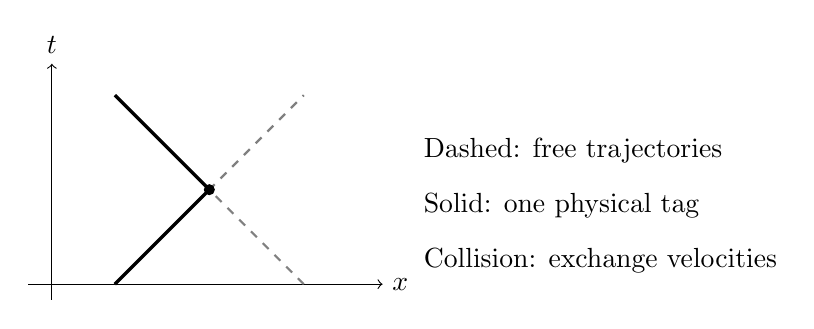
\begin{tikzpicture}[x=1cm,y=1cm]
\draw[->] (-0.3,0)--(4.2,0) node[right] {$x$};
\draw[->] (0,-0.2)--(0,2.8) node[above] {$t$};
\draw[gray,dashed,thick] (0.8,0)--(3.2,2.4);
\draw[gray,dashed,thick] (3.2,0)--(0.8,2.4);
\draw[very thick] (0.8,0)--(2,1.2)--(0.8,2.4);
\fill (2,1.2) circle (2pt);
\node[anchor=west] at (4.6,1.7) {Dashed: free trajectories};
\node[anchor=west] at (4.6,1.0) {Solid: one physical tag};
\node[anchor=west] at (4.6,0.3) {Collision: exchange velocities};
\end{tikzpicture}
\caption{One collision in the label-exchange construction. A physical tag
turns onto the other free line. Both preparations use this same rule.}
\label{fig:exchange}
\end{figure}

Place a typical particle at the origin at time zero and follow its position
$X(t)$. This selection is often called a Palm preparation. It fixes a tagged
origin without changing the macroscopic density. The velocity $V(t)$ and its
increments will have stationary statistics; the absolute position $X(0)=0$
is not itself a stationary random variable. Reflection symmetry gives
$\mathbb E[X(t)]=0$. We use the ordinary diffusion coefficient
\begin{equation}
 D=\lim_{t\to\infty}\frac{\Var X(t)}{2t},
 \label{eq:D}
\end{equation}
when the limit exists. Its units are length squared per time.

Both gases are defined on the infinite line before taking this limit. They
have finite energy density $\rho m u^2/2$, but infinite total reservoir energy.
On any finite time interval $[0,T]$, bounded speed confines the tag to
$[-uT,uT]$. Only free lines starting in $[-2uT,2uT]$ can affect it during that
interval. Local finiteness of either preparation therefore gives a well-defined
path with finitely many collisions. A finite container followed to arbitrarily
late times would be a different problem.

\section{Poisson gaps give an exponential collision clock}
For the first preparation, put independent Poisson particles of density $\rho$
on the line and give each an independent, equally probable velocity sign.
For a typical tag at zero the remaining gas has that same Poisson law.
The two velocity streams are independent Poisson processes of density
$\rho/2$. Free evolution translates each stream, preserving this homogeneous
marked configuration law.

Condition on an initially right-moving tag. Let $B_j$ be the initial positions
of successive left-moving lines to its right, and $-A_j$ those of successive
right-moving lines to its left, with $A_0=B_0=0$.
The tag follows $ut$, then $B_1-ut$, then $-A_1+ut$, then $B_2-ut$, and so on.
Parallel lines never intersect. At each reversal the next opposing line is
the next unused line in the corresponding ordered sequence. The collision
times consequently satisfy
\begin{equation}
 t_{2j-1}=\frac{B_j+A_{j-1}}{2u},\qquad
 t_{2j}=\frac{B_j+A_j}{2u}. \label{eq:times}
\end{equation}
Poisson gaps $B_j-B_{j-1}$ and $A_j-A_{j-1}$ are independent exponentials
with rate $\rho/2$. Dividing them by the relative speed $2u$ shows that all
tagged waiting times are independent exponentials with rate
\begin{equation}
 \lambda=\rho u. \label{eq:rate}
\end{equation}
Reflection handles the other initial sign. The tag is therefore a stationary
symmetric two-state velocity process, reversing at the times of a Poisson
process. This is the standard telegraph velocity law, now obtained from
spatial gaps rather than prescribed as a random clock.

If $N(s)$ counts reversals in a duration $s$, then
$V(s)=V(0)(-1)^{N(s)}$. Summing the Poisson probabilities gives
\begin{equation}
 C(s)=\mathbb E[V(0)V(s)]=u^2e^{-2\lambda s}. \label{eq:cov}
\end{equation}
Stationarity and $X(t)=\int_0^t V(r)\,dr$ imply
\begin{align}
 \Var X(t)&=2\int_0^t(t-s)C(s)\,ds\notag\\
 &=\frac{u^2}{\lambda}\left[t-
 \frac{1-e^{-2\lambda t}}{2\lambda}\right]. \label{eq:poissonvar}
\end{align}
Thus
\begin{equation}
 D_{\mathrm P}=\frac{u^2}{2\lambda}=\frac{u}{2\rho}>0. \label{eq:DP}
\end{equation}
The covariance and Markov interpretation agree with the exact two-speed
result of Balakrishnan, Bena and Van den Broeck.\cite{BalakrishnanBenaVanDenBroeck2002}
The tag here starts at one of the two gas velocities; a tag initially at rest
has a different transient law.

\section{Ordered streams give periodic cancellation}
For the second preparation set $a=2/\rho$. Right-moving free lines start at
$a\mathbb Z+U_+$ and left-moving lines at $a\mathbb Z+U_-$, where the two
phases are independent and uniform on $[0,a)$. Each stream has density
$1/a=\rho/2$. Space translations and free time evolution translate the two
phases modulo $a$, preserving their uniform joint law. This is another
stationary marked gas with the same one-particle velocity probabilities and
energy density. It changes both spatial gaps and their correlations with
velocity signs: the union is not a Poisson gas with independent marks.

A typical tag has either velocity sign with probability $1/2$. Conditional
on positive sign and placing it at zero, its own stream is $a\mathbb Z$;
the opposite stream retains an independent uniform phase $U\in(0,a)$.
Equation~\eqref{eq:times} now has
\begin{equation}
 A_j=ja,\qquad B_j=U+(j-1)a.
\end{equation}
The first waiting time $R=U/(2u)$ is uniform on $(0,d)$, where
\begin{equation}
 d=\frac{a}{2u}=\frac{1}{\rho u}.
\end{equation}
Every subsequent waiting time is exactly $d$. The uniform initial sign and
uniform residual time make the velocity a stationary square wave of period
$2d$. It reverses indefinitely at mean rate $1/d=\rho u$, yet the tag travels
as far to the right as to the left in each full period. Every realization
returns to its initial position after $2d$.

The variance can be computed without invoking a long-time correlation integral.
For $0\le s\le d$, there is no reversal with probability $1-s/d$, giving
a displacement of magnitude $us$. Otherwise a reversal at residual time
$r\in(0,s)$ gives displacement of magnitude $u|2r-s|$. Hence
\begin{align}
 \Var X(s)&=u^2\left[(1-s/d)s^2+
 \frac{1}{d}\int_0^s(2r-s)^2\,dr\right]\notag\\
 &=u^2\left(s^2-\frac{2s^3}{3d}\right). \label{eq:ordervar}
\end{align}
For any $t>0$, write $\delta=t-2d\lfloor t/(2d)\rfloor$ and
$s=\min(\delta,2d-\delta)$. Full periods contribute zero displacement.
Stationarity and cancellation over a full period equate the variance over
$\delta>d$ to that over its complementary duration $2d-\delta$.
Equation~\eqref{eq:ordervar} therefore gives $\Var X(t)$ with this folded $s$.
Its maximum, at $s=d$, is $u^2d^2/3$, so
\begin{equation}
 0\le\Var X(t)\le\frac{1}{3\rho^2},\qquad D_{\mathrm O}=0. \label{eq:DO}
\end{equation}
There is no disorder-driven diffusion hidden at a longer timescale: the paths
are exactly periodic. Simultaneous collisions elsewhere in the lattice are
disjoint binary events. Coincident initial phases have probability zero.

\section{What the comparison teaches}
Table~\ref{tab:comparison} collects the controlled quantities and the changed
preparation. Equal values of a mean waiting time and velocity variance do
not determine the covariance history that enters Eq.~\eqref{eq:poissonvar}.
In the ordered gas the initial global phases persist. The velocity process
is stationary but not mixing, and positive and negative displacements cancel
exactly. Inferring an effective independent collision clock from the mean
collision rate would discard precisely the information responsible for
Eq.~\eqref{eq:DO}.

\begin{table}[ht]
\centering\small
\begin{tabular}{@{}p{0.30\textwidth}p{0.31\textwidth}p{0.31\textwidth}@{}}
\toprule
Quantity & Poisson gas & Ordered streams\\
\midrule
Mass; speed; density & $m$; $u$; $\rho$ & $m$; $u$; $\rho$\\
Energy per length & $\rho mu^2/2$ & $\rho mu^2/2$\\
Velocity variance & $u^2$ & $u^2$\\
Mean collision rate & $\rho u$ & $\rho u$\\
Joint preparation & Poisson gaps; independent signs & Two shifted lattices; sign fixed by stream\\
Complete waiting intervals & Independent exponential, mean $d$ & Constant $d$\\
First residual interval & Exponential, mean $d$ & Uniform on $(0,d)$\\
Tagged displacement & Diffusive at long times & Bounded and periodic\\
Diffusion coefficient & $u/(2\rho)$ & $0$\\
\bottomrule
\end{tabular}
\caption{Same mechanics and mean collision frequency, different transport.
Here $d=1/(\rho u)$. The residual interval is measured from a typical observation
time, which need not coincide with a collision.}
\label{tab:comparison}
\end{table}

The distinction between a complete waiting interval and its residual provides
a useful teaching check. In the ordered gas the latter has mean $d/2$,
although collisions occur at long-run rate $1/d$. Taking the reciprocal of
the mean forward waiting time would give the wrong collision rate. In the
Poisson gas memorylessness makes those two means equal.

Three short classroom questions follow directly from the construction:
(i) derive Eq.~\eqref{eq:times} from a position--time diagram;
(ii) explain why the collision rate counts reversals rather than the rate
$2\lambda$ in the velocity covariance; and (iii) use a uniformly chosen
observation phase to derive the ordered residual law and verify cancellation
over a full period. Together these separate collision mechanics, spatial
statistics and transport, using only elastic collisions, exponential waiting
times and elementary integration.

\begin{thebibliography}{9}
\bibitem{BalakrishnanBenaVanDenBroeck2002}
V. Balakrishnan, I. Bena, and C. Van den Broeck,
``Velocity correlations, diffusion, and stochasticity in a one-dimensional
system,'' Phys. Rev. E \textbf{65}, 031102 (2002),
\href{https://doi.org/10.1103/PhysRevE.65.031102}{doi:10.1103/PhysRevE.65.031102}.
\bibitem{LeibovichBarkai2013}
N. Leibovich and E. Barkai,
``The lasting effect of initial conditions on single file diffusion,''
Phys. Rev. E \textbf{88}, 032107 (2013),
\href{https://doi.org/10.1103/PhysRevE.88.032107}{doi:10.1103/PhysRevE.88.032107}.
\bibitem{CividiniKundu2017}
J. Cividini and A. Kundu,
``Tagged particle in single-file diffusion with arbitrary initial conditions,''
arXiv:1704.04017 (2017),
\href{https://doi.org/10.1088/1742-5468/aa75de}{doi:10.1088/1742-5468/aa75de}.
\end{thebibliography}
\end{document}
